\documentclass[preprint,12pt,authoryear]{elsarticle}

\usepackage{amssymb}
\usepackage{amsmath}
\usepackage{booktabs}
\usepackage{tabularx}
\usepackage{array}
\usepackage{url}
\usepackage[hidelinks]{hyperref}

\journal{Computer Vision Review}

\newcommand{\placeholderfigure}[3]{%
\begin{figure}[t]
\centering
\fbox{\begin{minipage}{0.90\linewidth}\centering\vspace{0.8em}#3\vspace{0.8em}\end{minipage}}
\caption{#1}
\label{#2}
\end{figure}}

\begin{document}

\begin{frontmatter}

\title{Open-Vocabulary and Reasoning Segmentation with Vision-Language Foundation Models: A Survey}

\author{Author Name}
\affiliation{organization={School or Department},
            addressline={University or Institution},
            city={},
            postcode={},
            state={},
            country={}}

\begin{abstract}
This survey outline reviews open-vocabulary and reasoning segmentation with vision-language foundation models. The planned manuscript follows the transition from closed-set segmentation to CLIP-based open-vocabulary segmentation, promptable segmentation with SAM, unified vision-language decoding, and multimodal large language model based reasoning segmentation and pixel grounding. The final manuscript will emphasize method taxonomy, datasets, evaluation metrics, advantages, limitations, and future challenges across representative work from 2023 to 2025.
\end{abstract}

\begin{highlights}
\item The survey is organized around technical routes rather than a paper-by-paper chronology.
\item The core comparison covers CLIP-based OVSS, diffusion-based segmentation, SAM-based prompting, unified decoders, and MLLM-based reasoning segmentation.
\item The outline records where each section should discuss content, figures, datasets, metrics, and cross-method limitations.
\end{highlights}

\begin{keyword}
Open-vocabulary segmentation \sep reasoning segmentation \sep vision-language models \sep SAM \sep CLIP \sep pixel grounding
\end{keyword}

\end{frontmatter}

\section{Introduction}

Dense visual prediction is a central problem in computer vision, because scene understanding often requires semantic labels, object identities, or structured regions at the pixel level. Representative milestones such as Fully Convolutional Networks (FCNs)~\citep{long2015fully}, Mask R-CNN~\citep{he2017mask}, and panoptic segmentation~\citep{kirillov2019panoptic} helped establish stable benchmarks and reliable task-specific pipelines under a closed-set paradigm, where the label space is fixed during training and unchanged at test time. Nevertheless, this paradigm leaves three limitations that are increasingly restrictive. It struggles with unseen categories and fine-grained concepts, it depends on costly dense mask annotation, and it cannot express user intents that are naturally described through free-form language.

Vision-language models (VLMs) offer a way to relax these restrictions by aligning visual regions with textual concepts. Contrastive Language-Image Pre-training (CLIP)~\citep{radford2021learning} showed that large-scale image-text supervision can support transferable visual recognition, which encouraged dense prediction systems to move from fixed labels toward text-defined category recognition. Early open-vocabulary segmentation methods, including Mask-adapted CLIP~\citep{liang2023ovseg}, Side Adapter Network (SAN)~\citep{xu2023san}, Open-Vocabulary Panoptic Segmentation with Text-to-Image Diffusion Models (ODISE)~\citep{xu2023odise}, and related recent studies~\citep{xshanOpenvocabularySemanticSegmentation2024,xwangUseUniversalSegment2024,shinhOpenvocabularySemanticSegmentation2024,yxchngAligningVisionLanguageModel2026}, transfer image-text semantics to pixels so that segmentation systems can recognize categories beyond the training label set. Yet semantic openness alone does not solve dense prediction. Open-vocabulary segmentation must preserve broad VLM semantics while recovering accurate boundaries, small structures, and region-level distinctions, which creates a persistent tension between semantic breadth and spatial precision.

\begin{figure}[t]
    \centering
    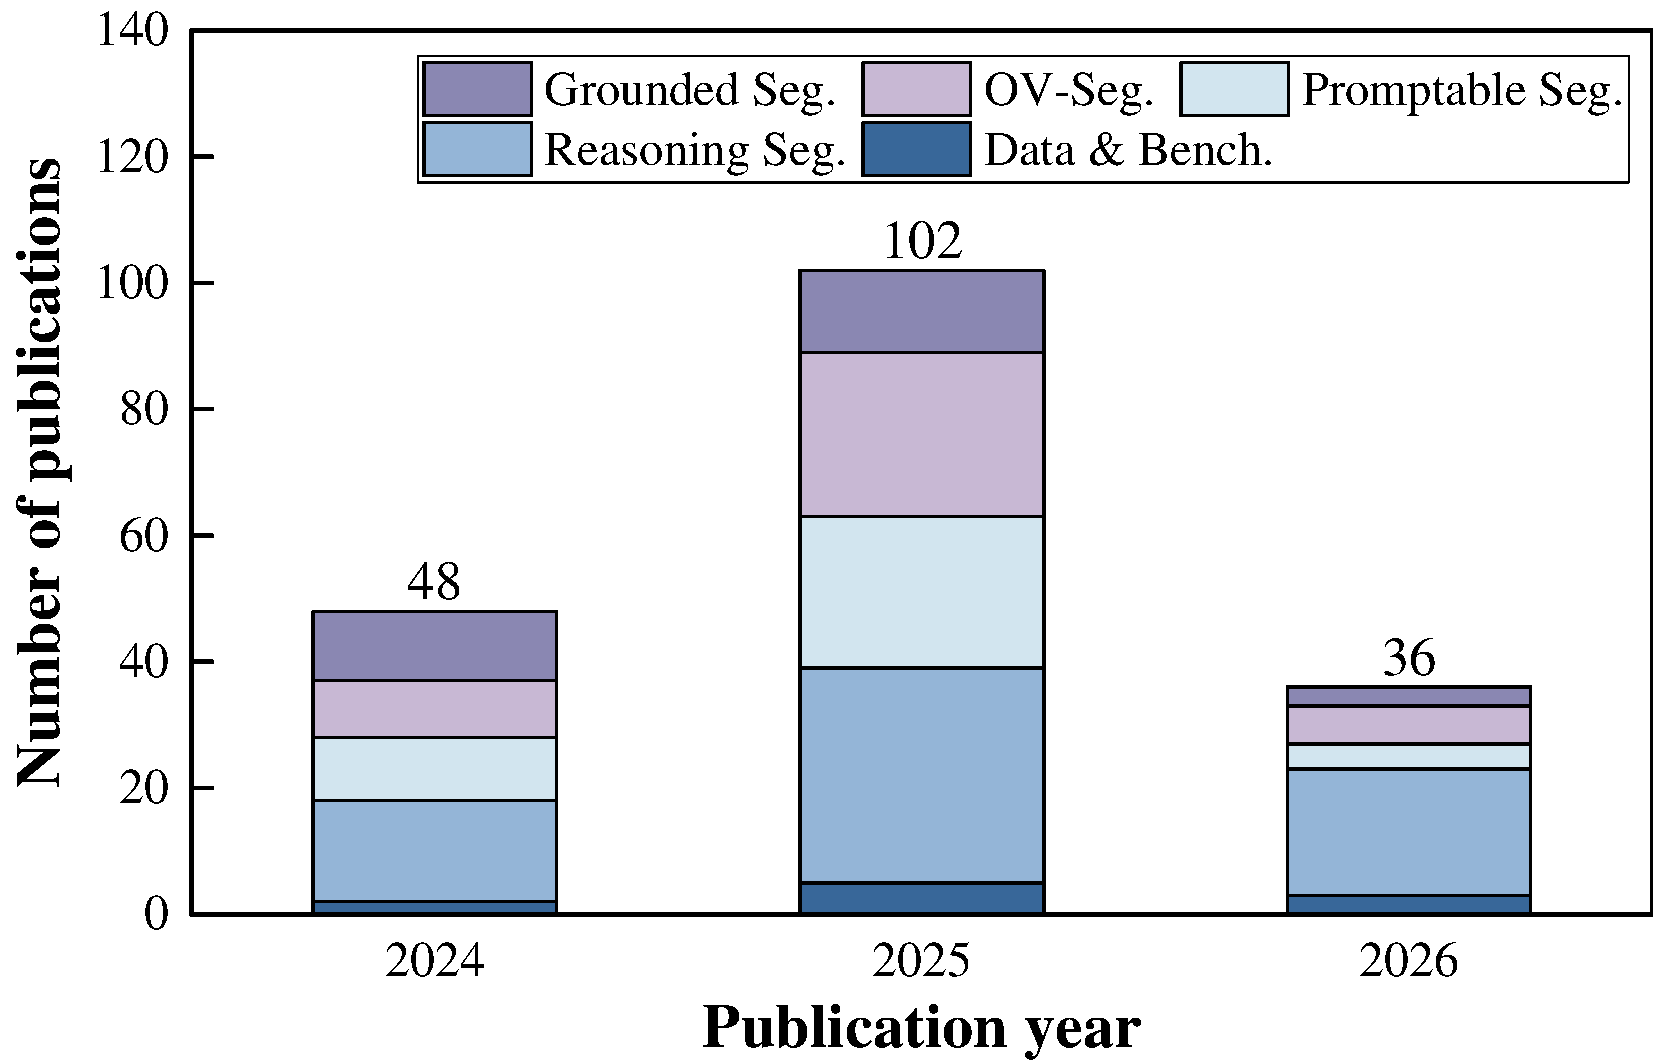
\includegraphics[width=0.85\linewidth]{Fig/Numberofpublications.pdf}
    \caption{Number of publications in the curated survey corpus from 2024 to 2026. The stacked bars group papers into grounded segmentation, reasoning segmentation, open-vocabulary segmentation, data and benchmarks, and promptable segmentation.}
    \label{fig-publication-statistics}
\end{figure}

\begin{figure*}[!t]
    \centering
    \includegraphics[width=0.98\textwidth]{Fig/intro_overview.png}
    \caption{Overview and taxonomy of the field evolution and technical routes reviewed in this survey. The top row summarizes the transition from closed-set segmentation to open-vocabulary, promptable, unified vision-language, and reasoning segmentation. The middle row groups the core technical routes. The bottom row places representative methods along the temporal development.}
    \label{fig-intro-overview}
\end{figure*}

Recent work has therefore developed several complementary routes. CLIP-based dense alignment adapts image-text representations to pixel prediction, proposal-then-classification pipelines classify candidate regions or masks, and the Segment Anything Model (SAM)~\citep{kirillov2023sam} together with Segment Anything Model 2 (SAM2)~\citep{ravi2024sam2} provides class-agnostic mask priors that separate mask generation from semantic assignment. SAM-based systems such as X-SAM~\citep{hwangXSAMSegmentAnything2026} and OpenWorldSAM~\citep{sgxiaoOpenworldsamExtendingSam22026} further extend promptable masks toward broader segmentation settings. In parallel, region-word and mask-text grounding methods connect linguistic units with spatial masks, supporting referring expression segmentation, grounded conversation, and fine-grained pixel-level visual understanding~\citep{xuPixelalignedLanguageModel2024,zhangLlavagroundingGroundedVisual2024,youFerretReferGround2024,rasheedGlammPixelGrounding2024}. These routes show that the field is no longer defined only by category recognition, but also by how language is grounded into spatial evidence.


The field has also shifted from naming visible categories to reasoning about what should be segmented. In reasoning segmentation, a query may refer to an implicit target through commonsense, spatial relations, multi-step instructions, false premises, or domain rules. Multimodal large language models (MLLMs) such as Large Language Instructed Segmentation Assistant (LISA)~\citep{lai2024lisa}, PixelLM~\citep{renPixellmPixelReasoning2024}, and Pixel Grounding Large Multimodal Model (GLaMM)~\citep{rasheed2024glamm} connect language generation with mask prediction through segmentation tokens, pixel decoders, or grounded multimodal conversation. Newer work further explores agentic reasoning, reinforcement learning (RL), preference optimization, and verifiable grounding to improve instruction following and mask faithfulness~\citep{luoConnectingDotsTrainingFree2026,zhuLensLearningSegment2026,zhouReasoningImplicitSelfsupervised2026,guoSeeingBelievingRichContext2026}. This shift expands segmentation into an interface where visual perception, language grounding, and structured reasoning must be modeled together.



The rapid concentration of recent work motivates a systematic review. As shown in Fig.~\ref{fig-publication-statistics}, the curated corpus contains 48 papers from 2024, 102 from 2025, and 36 from 2026, spanning open-vocabulary segmentation, promptable segmentation, grounded segmentation, reasoning segmentation, and dataset or benchmark construction. This distribution reflects a change in the center of gravity. Earlier studies emphasized text-defined labels and dense semantic alignment, whereas recent work increasingly targets promptable mask generation, instruction-guided segmentation, grounded multimodal dialogue, and reasoning-intensive pixel grounding. A survey is therefore needed to explain not only the growth of the literature, but also the technical routes that make these tasks comparable.

Fig.~\ref{fig-intro-overview} summarizes the taxonomy adopted in this survey. Across method families, the common system is composed of visual and textual representations that define the semantic space, mask generators or decoders that produce spatial regions, region or mask-text alignment mechanisms that bind language to pixels, and evaluation protocols that test openness, grounding, and reasoning. Based on these components, we organize the literature around technical routes rather than a paper-by-paper chronology. Open-vocabulary segmentation studies focus on dense semantic alignment, mask classification, and efficient adaptation. Promptable and grounded segmentation studies combine mask priors, region-word alignment, and language-guided prompting. Reasoning segmentation studies introduce MLLMs, explicit reasoning traces, grounded dialogue, and optimization with RL. Extended scenarios in video, 3D, remote sensing, medicine, affordance, and embodied grounding test whether these systems generalize beyond static 2D natural images~\citep{xuVideosegr1ReasoningVideo2026,chen3DDRESDetailed3D2026,libExploringEfficientOpenvocabulary2026,yanMedreasonerReinforcementLearning2026,wangAffordancer1ReinforcementLearning2026}.

Despite this progress, the literature remains difficult to compare. Different studies assume different prompt formats, label spaces, mask generators, training data, foundation backbones, and evaluation metrics. Some works evaluate open-vocabulary semantic segmentation with class-level labels, whereas others evaluate referring or reasoning segmentation with sentence-level instructions, mask-text pairs, or grounded conversations. Benchmark fragility further complicates comparison, because dataset names and label vocabularies may bias open-vocabulary evaluation, domain-specific imagery creates additional gaps, and MLLM outputs may be linguistically plausible but visually ungrounded~\citep{hhuangRenovatingNamesOpenvocabulary2024,libExploringEfficientOpenvocabulary2026,guoSeeingBelievingRichContext2026}. A useful survey must therefore clarify what methods exist, what each method assumes, what evidence supports its claimed capability, and where comparisons are not yet fair. We center this review on three recurring tensions, including semantic openness versus spatial precision, prompt and reasoning flexibility versus grounding faithfulness, and benchmark diversity versus fair comparison.

This survey provides a structured view of open-vocabulary and reasoning segmentation with vision-language foundation models. Its contributions are fourfold. First, we trace the development from closed-set dense prediction to open-vocabulary, promptable, grounded, and reasoning segmentation, clarifying the task assumptions behind each paradigm. Second, we summarize the common foundations, datasets, annotation granularity, and evaluation protocols that govern fair comparison. Third, we organize recent methods into technical families covering CLIP-based dense alignment, proposal and mask classification, SAM-based prompting with SAM2 extensions, region-word and mask-text grounding, MLLM-guided segmentation, and reasoning-to-mask generation. Fourth, we compare cross-family assumptions, benchmark settings, and trade-offs, then derive future directions on unified evaluation, faithful grounding, efficient adaptation, and generalization beyond static 2D natural images.

The rest of this survey is organized as follows. Section~2 introduces the background and task evolution. Section~3 presents the foundations of visual, textual, and mask representations. Section~4 reviews datasets, annotation types, and evaluation protocols. Sections~5 to~7 survey open-vocabulary segmentation, promptable and grounded segmentation, and reasoning segmentation. Section~8 discusses extended scenarios including video, 3D, remote sensing, medicine, affordance, and embodied grounding. Section~9 compares method families and benchmark limitations. Section~10 outlines future directions, and Section~11 concludes the survey.

\section{Background and Objective}
\label{sec:background}

\subsection{Closed-set segmentation and its limitation}
\label{subsec:closed-set}
Writing plan: define the classical dense prediction tasks before introducing open-vocabulary methods. The goal is to clarify what changes when segmentation is no longer restricted to a fixed label set.

\subsubsection{Semantic segmentation}
\label{subsubsec:semantic-segmentation}
Explain that semantic segmentation assigns one class label to each pixel. It is suitable for scene parsing but does not distinguish different instances of the same category.

\subsubsection{Instance segmentation}
\label{subsubsec:instance-segmentation}
Explain that instance segmentation predicts object-level masks and instance identities, but it normally assumes a predefined set of object categories.

\subsubsection{Panoptic segmentation}
\label{subsubsec:panoptic-segmentation}
Explain that panoptic segmentation unifies thing and stuff prediction. Use ODISE as the later open-vocabulary panoptic example \citep{xu2023odise}.

\subsection{Open-vocabulary segmentation}
\label{subsec:open-vocabulary-background}
Writing plan: define open-vocabulary semantic segmentation as dense classification over categories that may not appear in the segmentation training set. Emphasize that text prompts or category names provide the label space at inference time.

\subsubsection{Text-defined label spaces}
\label{subsubsec:text-defined-labels}
Explain how category names or prompt templates become text embeddings. This should prepare the reader for CLIP-based methods such as OVSeg and SAN \citep{liang2023ovseg,xu2023san}.

\subsubsection{Zero-shot and cross-dataset transfer}
\label{subsubsec:zero-shot-transfer}
Explain that open-vocabulary performance is usually measured by transferring from one training dataset to unseen datasets such as ADE20K, PASCAL VOC, PASCAL Context, and COCO-Stuff. Note that mIoU remains common but does not fully capture vocabulary ambiguity.

\subsection{Reasoning segmentation and pixel grounding}
\label{subsec:reasoning-background}
Writing plan: introduce the shift from category names to complex natural-language instructions. The key distinction is that the target object may be implicit and must be inferred from language, commonsense, scene context, or conversation.

\subsubsection{Referring segmentation versus reasoning segmentation}
\label{subsubsec:referring-vs-reasoning}
Explain that referring segmentation usually localizes an explicitly described object, whereas reasoning segmentation may require implicit constraints such as ``the object that the man is holding''. LISA should be introduced here as the representative reasoning segmentation method \citep{lai2024lisa}.

\subsubsection{Pixel grounding in multimodal conversation}
\label{subsubsec:pixel-grounding}
Explain that pixel grounding connects generated words, phrases, or entities to masks. GLaMM should be positioned as the representative grounded conversation method \citep{rasheed2024glamm}.

\placeholderfigure{Planned background figure: task hierarchy from closed-set segmentation to open-vocabulary segmentation, referring segmentation, reasoning segmentation, and grounded conversation.}{fig:background-task-hierarchy}{Figure plan: show how the input changes from a fixed class list, to text labels, to referring expressions, to reasoning queries and multimodal dialogue.}
\section{Method Taxonomy}
\label{sec:method-taxonomy}

\subsection{CLIP-based open-vocabulary segmentation}
\label{subsec:clip-based-ovss}
Writing plan: explain why CLIP is attractive for open-vocabulary segmentation and why direct CLIP application is insufficient for pixel-level prediction. The central tension is strong image-text alignment versus weak dense localization.

\subsubsection{Mask-adapted region classification}
\label{subsubsec:mask-adapted-clip}
Discuss OVSeg as the canonical two-stage route: class-agnostic mask proposal followed by mask-adapted CLIP classification \citep{liang2023ovseg}. Explain the masked-region distribution shift and why mask prompt tuning or adaptation is needed.

\subsubsection{Efficient side adaptation}
\label{subsubsec:side-adapter}
Discuss SAN as an efficient alternative to repeated proposal classification. Emphasize the side adapter, attention bias, and proposal-wise recognition with a mostly frozen CLIP backbone \citep{xu2023san}.

\subsubsection{Training-free VLM feature mining}
\label{subsubsec:pnp-ovss}
Discuss PnP-OVSS as a 2024 training-free route that mines localization cues from off-the-shelf VLMs \citep{luo2024pnpovss}. Explain the advantage of removing task-specific segmentation training and the limitation of heuristic sensitivity.

\placeholderfigure{Planned figure: comparison of CLIP-based OVSS pipelines.}{fig:clip-ovss-pipelines}{Figure plan: redraw three columns for OVSeg, SAN, and PnP-OVSS: proposal-classification, side-adapter recognition, and training-free feature mining.}

\subsection{Diffusion-based open-vocabulary segmentation}
\label{subsec:diffusion-ovss}
Writing plan: introduce the idea that text-to-image diffusion models learn spatially meaningful intermediate representations, which can be repurposed for discriminative segmentation.

\subsubsection{Diffusion features as spatial-semantic representations}
\label{subsubsec:diffusion-features}
Discuss why the internal UNet features of text-to-image diffusion models can contain object- and part-level semantics. Use ODISE as the main example \citep{xu2023odise}.

\subsubsection{Combining generative and discriminative components}
\label{subsubsec:diffusion-discriminative}
Explain how ODISE combines frozen diffusion features, a mask generator, and CLIP-based text classification for open-vocabulary panoptic segmentation \citep{xu2023odise}.

\subsubsection{Strengths and costs}
\label{subsubsec:diffusion-costs}
Summarize the main advantage as broad spatial-semantic knowledge and the main limitation as high training and inference cost.

\placeholderfigure{Planned figure: ODISE-style diffusion feature pipeline.}{fig:odise-pipeline}{Figure plan: show a text-to-image diffusion UNet feeding a mask decoder and a text-conditioned open-vocabulary classifier.}

\subsection{Promptable segmentation foundation models}
\label{subsec:promptable-sam}
Writing plan: present SAM as the foundation model that changes segmentation from category prediction to prompt-conditioned mask generation \citep{kirillov2023sam}.

\subsubsection{SAM and promptable segmentation}
\label{subsubsec:sam-promptable}
Explain point, box, and mask prompts; the image encoder, prompt encoder, and mask decoder; and the SA-1B data engine \citep{kirillov2023sam}. Stress that SAM produces high-quality class-agnostic masks rather than semantic labels.

\subsubsection{SAM-enhanced open-vocabulary segmentation}
\label{subsubsec:sam-enhanced-ovss}
Discuss ESC-Net as a 2025 example that embeds SAM decoder blocks into one-stage OVSS while retaining CLIP-based category semantics \citep{lee2025escnet}. The section should explain how SAM supplies spatial priors while CLIP supplies text-category alignment.

\subsubsection{Training-free VFM composition}
\label{subsubsec:vfm-composition}
Discuss Trident as a 2025 training-free foundation-model composition route, combining complementary signals such as CLIP, DINO, and SAM \citep{shi2025trident}. Highlight the trade-off between no task-specific training and multi-model inference complexity.

\placeholderfigure{Planned figure: SAM and SAM-derived OVSS routes.}{fig:sam-routes}{Figure plan: start from SAM's image encoder, prompt encoder, and mask decoder, then branch to ESC-Net's CLIP-SAM fusion and Trident's training-free CLIP/DINO/SAM composition.}

\subsection{Unified vision-language segmentation models}
\label{subsec:unified-vl-segmentation}
Writing plan: explain why unified decoders are an intermediate stage between specialized segmentation models and MLLM-based reasoning systems.

\subsubsection{Pixel, image, and language outputs in one decoder}
\label{subsubsec:xdecoder-unified-output}
Discuss X-Decoder as a generalized decoder for segmentation, referring, retrieval, captioning, and VQA transfer \citep{zou2023xdecoder}. Explain how pixel-level and language-level outputs are represented in a shared model.

\subsubsection{Generic queries and semantic queries}
\label{subsubsec:xdecoder-queries}
Explain generic queries, text queries, and semantic query interaction. This part should clarify why X-Decoder is broader than CLIP-based mask classification but still different from MLLM reasoning.

\subsubsection{Transition toward generalist vision-language models}
\label{subsubsec:xdecoder-transition}
Position X-Decoder as a bridge: it unifies dense and language tasks, but it does not provide the same free-form reasoning and grounded conversation interface as LISA or GLaMM \citep{lai2024lisa,rasheed2024glamm,zou2023xdecoder}.

\placeholderfigure{Planned figure: generalized decoding in X-Decoder.}{fig:xdecoder-generalized}{Figure plan: redraw an image encoder, text encoder, and shared decoder with outputs for segmentation masks, retrieval embeddings, captions, and VQA responses.}

\subsection{MLLM-based reasoning segmentation and pixel grounding}
\label{subsec:mllm-reasoning}
Writing plan: describe the shift from text labels to complex instructions. The key question is how a language token or generated phrase becomes a pixel mask.

\subsubsection{Reasoning segmentation with segmentation tokens}
\label{subsubsec:lisa-seg-token}
Discuss LISA's use of a special segmentation token and its hidden embedding to drive a mask decoder \citep{lai2024lisa}. Explain the role of MLLM understanding, SAM-style segmentation backends, and instruction-formatted training data.

\subsubsection{Grounded conversation generation}
\label{subsubsec:glamm-grounded-conversation}
Discuss GLaMM as a grounded multimodal model that links generated phrase-level entities to pixel masks \citep{rasheed2024glamm}. Contrast this with single-target reasoning segmentation.

\subsubsection{Risks: hallucination, evaluation, and mask precision}
\label{subsubsec:mllm-risks}
Explain that MLLM-based methods can understand richer language but introduce hallucination risk, heavier training and inference, and more complex evaluation. The subsection should separate reasoning correctness from boundary accuracy.

\placeholderfigure{Planned figure: MLLM-to-mask mechanisms.}{fig:mllm-to-mask}{Figure plan: compare LISA's segmentation-token-to-mask path with GLaMM's phrase-level grounded conversation path.}

\subsection{Extensions to video, 3D, and complex scenes}
\label{subsec:video-3d-extensions}
Writing plan: keep this subsection shorter because the local ten-paper set mainly covers 2D image segmentation. Use it as a forward-looking bridge to video reasoning segmentation, 3D or multiview grounding, and multi-context visual grounding.

\subsubsection{Video reasoning segmentation}
\label{subsubsec:video-reasoning}
Explain that video adds temporal consistency, object persistence, motion cues, and memory. Add VRS-HQ or GLUS citations after their source files are added to the project bibliography.

\subsubsection{3D and multiview grounding}
\label{subsubsec:three-d-grounding}
Explain that 3D and multiview scenes require spatial consistency across views, camera poses, and object instances. This should be treated as an extension of pixel grounding beyond single images.

\subsubsection{Complex multi-context scenes}
\label{subsubsec:multi-context-scenes}
Explain that multi-image or multi-context grounding stresses MLLM reasoning and object disambiguation. Add MC-Bench or related citations after the corresponding source files are included.

\placeholderfigure{Planned figure: extension path from image segmentation to video, 3D, and multi-context grounding.}{fig:extensions}{Figure plan: draw image, video, 3D/multiview, and multi-context settings, with the added challenge under each setting.}
\section{Datasets and Evaluation Metrics}
\label{sec:datasets-metrics}

\subsection{Dataset groups}
\label{subsec:dataset-groups}
Writing plan: group datasets by task rather than listing them alphabetically. The tables should show how each dataset supports a different part of the survey argument.

\begin{table}[t]
\centering
\small
\caption{Core datasets for open-vocabulary and promptable segmentation.}
\label{tab:datasets-core}
\begin{tabularx}{\linewidth}{p{0.18\linewidth} p{0.23\linewidth} p{0.25\linewidth} X}
\toprule
Dataset & Task & Used by & Main property \\
\midrule
SA-1B & Promptable segmentation & SAM \citep{kirillov2023sam} & Large-scale class-agnostic mask data. \\
ADE20K & Scene parsing and OVSS & SAN, ODISE, ESC-Net, Trident \citep{xu2023san,xu2023odise,lee2025escnet,shi2025trident} & Rich scene categories for open-vocabulary transfer. \\
PASCAL VOC & Semantic segmentation & OVSS methods \citep{liang2023ovseg,xu2023san,luo2024pnpovss} & Compact and common zero-shot benchmark. \\
PASCAL Context & Semantic segmentation & OVSS methods \citep{liang2023ovseg,xu2023san} & Broader dense semantic labels than VOC. \\
COCO-Stuff & Semantic segmentation & OVSS training and evaluation \citep{xu2023san,liang2023ovseg} & Stuff categories and dense scene labels. \\
COCO Panoptic & Panoptic segmentation & ODISE, X-Decoder \citep{xu2023odise,zou2023xdecoder} & Joint thing and stuff annotation. \\
\bottomrule
\end{tabularx}
\end{table}

\begin{table}[t]
\centering
\small
\caption{Datasets for language-guided, reasoning, grounding, and future video settings.}
\label{tab:datasets-grounding}
\begin{tabularx}{\linewidth}{p{0.22\linewidth} p{0.22\linewidth} p{0.24\linewidth} X}
\toprule
Dataset & Task & Used by & Main property \\
\midrule
RefCOCO / RefCOCO+ / RefCOCOg & Referring segmentation & LISA, GLaMM, X-Decoder \citep{lai2024lisa,rasheed2024glamm,zou2023xdecoder} & Language-guided object masks. \\
ReasonSeg & Reasoning segmentation & LISA \citep{lai2024lisa} & Complex implicit queries requiring reasoning. \\
GranD / GranDf & Grounded conversation & GLaMM \citep{rasheed2024glamm} & Phrase-level masks for generated responses. \\
Video reasoning datasets & Video reasoning segmentation & Future video extensions & Temporal masks and consistency requirements. \\
\bottomrule
\end{tabularx}
\end{table}

\subsection{Evaluation metrics}
\label{subsec:evaluation-metrics}
Writing plan: separate segmentation quality, open-vocabulary transfer, reasoning correctness, and computational cost. The final text should avoid treating all methods as if they solve the same task.

\subsubsection{Dense segmentation metrics}
\label{subsubsec:dense-metrics}
Discuss mIoU for semantic segmentation, PQ for panoptic segmentation, and AP or mask AP for instance-level outputs. Connect mIoU to OVSeg, SAN, PnP-OVSS, ESC-Net, and Trident \citep{liang2023ovseg,xu2023san,luo2024pnpovss,lee2025escnet,shi2025trident}; connect PQ/AP to ODISE and X-Decoder \citep{xu2023odise,zou2023xdecoder}.

\subsubsection{Language-guided and reasoning metrics}
\label{subsubsec:reasoning-metrics}
Discuss cIoU, gIoU, and task-specific grounding scores for referring and reasoning segmentation. Explain that these metrics should be interpreted together with language correctness for LISA and GLaMM \citep{lai2024lisa,rasheed2024glamm}.

\subsubsection{Efficiency and deployment metrics}
\label{subsubsec:efficiency-metrics}
Discuss FPS, GFLOPs, parameter count, memory, and multi-model inference cost. This is important for comparing SAN, PnP-OVSS, ESC-Net, and Trident \citep{xu2023san,luo2024pnpovss,lee2025escnet,shi2025trident}.

\placeholderfigure{Planned figure: dataset and metric map.}{fig:dataset-metric-map}{Figure plan: map each task family to datasets and metrics, so readers can see why mIoU alone is insufficient for reasoning segmentation and grounded conversation.}
\section{Comparison of Advantages and Shortcomings}
\label{sec:comparison}

\subsection{Cross-method comparison}
\label{subsec:cross-method-comparison}
Writing plan: this is the main synthesis section. Do not describe papers one by one. Compare assumptions, model inputs, supervision, output type, strengths, and weaknesses.

\begin{table}[t]
\centering
\small
\caption{Comparison of segmentation-centered method families.}
\label{tab:method-comparison-segmentation}
\begin{tabularx}{\linewidth}{p{0.20\linewidth} p{0.25\linewidth} X X}
\toprule
Method type & Representative papers & Advantage & Shortcoming \\
\midrule
CLIP-based OVSS & OVSeg, SAN, PnP-OVSS \citep{liang2023ovseg,xu2023san,luo2024pnpovss} & Strong open-vocabulary semantics and natural zero-shot category transfer. & CLIP is not designed for dense localization; spatial precision and prompt sensitivity remain issues. \\
Diffusion-based segmentation & ODISE \citep{xu2023odise} & Diffusion features provide rich spatial-semantic representations and support panoptic output. & Training and inference are costly, and the system is more complex than lightweight CLIP adapters. \\
SAM and VFM-based methods & SAM, ESC-Net, Trident \citep{kirillov2023sam,lee2025escnet,shi2025trident} & High-quality masks and strong generalization from promptable or compositional foundation models. & Native semantic understanding is limited; additional CLIP, VLM, or MLLM components are required. \\
\bottomrule
\end{tabularx}
\end{table}

\begin{table}[t]
\centering
\small
\caption{Comparison of generalist, reasoning, and extension-oriented method families.}
\label{tab:method-comparison-generalist}
\begin{tabularx}{\linewidth}{p{0.20\linewidth} p{0.25\linewidth} X X}
\toprule
Method type & Representative papers & Advantage & Shortcoming \\
\midrule
Unified decoder models & X-Decoder \citep{zou2023xdecoder} & Pixel, image, and language tasks can be handled in one framework. & Training is data-hungry and task balancing is difficult. \\
MLLM-based reasoning segmentation & LISA, GLaMM \citep{lai2024lisa,rasheed2024glamm} & Complex natural-language instructions, commonsense reasoning, and pixel grounding become possible. & Hallucination, fine boundary accuracy, heavy training cost, and evaluation ambiguity remain major problems. \\
Video, 3D, and complex-scene extensions & To be added & Closer to real applications with temporal or spatial consistency. & Annotation cost, memory, computation, and consistency evaluation are harder than in single-image settings. \\
\bottomrule
\end{tabularx}
\end{table}

\subsection{Trade-off axes}
\label{subsec:tradeoff-axes}
Writing plan: summarize the survey using several axes: semantic openness, mask quality, reasoning complexity, training cost, inference cost, and extensibility.

\subsubsection{Semantic openness versus spatial precision}
\label{subsubsec:semantic-vs-spatial}
Compare CLIP-based methods with SAM-based methods. CLIP supplies open semantics but weak localization, whereas SAM supplies masks but lacks category-level semantics \citep{liang2023ovseg,xu2023san,kirillov2023sam}.

\subsubsection{Training-based adaptation versus training-free composition}
\label{subsubsec:training-vs-training-free}
Compare OVSeg, SAN, and ESC-Net with PnP-OVSS and Trident. The former can learn task-specific structure, while the latter reduces training cost but may depend on heuristic fusion and multiple off-the-shelf models \citep{liang2023ovseg,xu2023san,lee2025escnet,luo2024pnpovss,shi2025trident}.

\subsubsection{Task-specific segmentation versus generalist reasoning}
\label{subsubsec:specialist-vs-generalist}
Compare specialized OVSS models with X-Decoder, LISA, and GLaMM. The main point is that generality improves interaction and reasoning ability but complicates training, evaluation, and deployment \citep{zou2023xdecoder,lai2024lisa,rasheed2024glamm}.

\placeholderfigure{Planned figure: capability trade-off map.}{fig:capability-tradeoff}{Figure plan: plot methods on axes such as semantic openness, mask precision, reasoning ability, and computational cost.}
\section{Challenges and Future Directions}
\label{sec:future-directions}

\subsection{From open vocabulary to reliable open-world segmentation}
\label{subsec:reliable-open-world}
Writing plan: argue that recognizing unseen category names is not enough. Future systems must handle label ambiguity, synonyms, rare categories, domain shift, and negative prompts.

\subsection{Integrating semantic alignment and mask priors}
\label{subsec:semantic-mask-integration}
Writing plan: discuss why CLIP, SAM, DINO, diffusion, and MLLM components are often complementary. Use ESC-Net and Trident as examples of 2025 methods that explicitly combine foundation-model strengths \citep{lee2025escnet,shi2025trident}.

\subsection{Reducing hallucination in reasoning segmentation}
\label{subsec:hallucination-reasoning}
Writing plan: discuss hallucination and faithfulness in LISA- and GLaMM-style systems \citep{lai2024lisa,rasheed2024glamm}. Separate language plausibility from pixel-level correctness.

\subsection{Evaluation beyond mIoU}
\label{subsec:evaluation-beyond-miou}
Writing plan: argue that mIoU is insufficient for reasoning segmentation, grounded conversation, video, and 3D grounding. Future evaluation should include language faithfulness, grounding faithfulness, temporal consistency, and efficiency.

\subsection{Video, 3D, and multi-context grounding}
\label{subsec:future-video-3d}
Writing plan: describe temporal consistency, spatial consistency, and multi-context reasoning as natural extensions. Add citations for VRS-HQ, GLUS, MC-Bench, or related papers after those source files are incorporated into the local bibliography.

\placeholderfigure{Planned figure: open problems map.}{fig:open-problems}{Figure plan: organize future challenges by semantic complexity and spatial-temporal complexity, then place open-vocabulary segmentation, reasoning segmentation, video, 3D, and multi-context grounding on the map.}
\section{Conclusion}
\label{sec:conclusion}

Writing plan: close with a bounded synthesis. State that open-vocabulary and reasoning segmentation has moved from CLIP-based category transfer in 2023, through SAM and unified decoders, to MLLM-driven reasoning and pixel grounding in 2024--2025. Emphasize that current systems still face trade-offs among semantic openness, mask quality, reasoning reliability, computational cost, and extension to video or 3D scenes. The conclusion should not introduce new methods; it should summarize the taxonomy and the main open challenges.

\bibliographystyle{elsarticle-harv}
\bibliography{references}

\end{document}